\documentclass[10pt,letterpaper]{article}

\usepackage[utf8]{inputenc}
\usepackage[spanish,es-nodecimaldot]{babel}
\usepackage{amsmath}
\usepackage{amssymb}
\usepackage{graphicx}

\usepackage[most]{tcolorbox}

\usepackage{multicol}

\usepackage{mathtools}
\usepackage{forest}
\usepackage{tikz}
\usetikzlibrary{trees,positioning}

\usepackage[top=1in, bottom=1in, left=1in, right=1in]{geometry}


\begin{document}

\begin{titlepage}
    \centering

    {\scshape\LARGE Universidad Nacional Autónoma de México \par}

    \vspace{1cm}
    {\scshape\Large Facultad de Ciencias\par}
    \vspace{1.5cm}

    \begin{center}
        
\includegraphics[scale=.1]{../../../assets/img/logo.png}
    \end{center}

    \vspace{.8 cm}

    {\LARGE Boletín de Ejercicios 01: \par}
    {\huge\bfseries Primer parcial \par}

    \vspace{0.5cm}
    {\large\itshape Pablo A. Trinidad Paz\par}
    419004279

    \vfill

    Trabajo presentado como parte del curso de \textbf{Estructuras Discretas}
    impartido por la profesora \textbf{Pilar Selene Linares Arévalo}. \par
    \vspace{0.1cm}
    {\large 12 de Septiembre de 2018\par}
\end{titlepage}


\begin{enumerate}
    \item Considera la siguiente gramática
        \begin{equation*} \begin{split} \begin{aligned}
            &S :: = E \\
            &E :: = \downarrow E \uparrow \\
            &E :: = \bigcirc E \\
            &E :: = \uparrow \uparrow E \\
            &E :: = \square \alpha \\
            &E :: = \delta
        \end{aligned} \end{split} \end{equation*}

        \begin{enumerate}
            \item Construye una derivación correspondiente a la cadena
                  $\uparrow \uparrow \downarrow \bigcirc \uparrow \uparrow \square \alpha \uparrow$.

                \begin{center}
                    \begin{tikzpicture}[nodes={draw,circle}]
                        \node {$S$}
                        child {node {$E$}
                            child {node {$\uparrow \uparrow$}}
                            child {node {$E$}
                                child {node {$\downarrow$}}
                                child {node {$E$}
                                    child {node {$\bigcirc$}}
                                    child {node {$E$}
                                        child {node {$\uparrow \uparrow$}}
                                        child {node {$E$}
                                            child {node {$\square\alpha$}}
                                        }
                                    }
                                }
                                child {node {$\uparrow$}}
                            }
                        };
                    \end{tikzpicture}
                \end{center}

            \item Da el árbol que corresponde a la expresión $\bigcirc \downarrow \square \alpha \uparrow$.
                \begin{center}
                    \begin{tikzpicture}[nodes={draw, circle}]
                        \node {$S$}
                        child {node {$E$}
                            child {node {$\bigcirc$}}
                            child {node {$E$}
                                child {node {$\downarrow$}}
                                child {node {$E$}
                                    child {node {$\square\alpha$}}
                                }
                                child {node {$\uparrow$}}
                            }
                        };
                    \end{tikzpicture}
                \end{center}

            \clearpage
            \item ¿La cadena $\uparrow \uparrow \uparrow \bigcirc \delta$ está bien formada?
                  Justifique su respuesta.
                \begin{multicols}{2}
                    \begin{center}
                        \begin{tikzpicture}[nodes={draw, circle}]
                            \node {$S$}
                                child {node {$E$}
                                    child {node {$\uparrow \uparrow$}}
                                    child {node {$E$}}
                            };
                        \end{tikzpicture}
                    \end{center}
                    \begin{center}
                        \begin{tikzpicture}[nodes={draw, circle}]
                            \node {$S$}
                                child {node {$E$}
                                    child {node {$\uparrow \uparrow$}}
                                    child {node {$E$}
                                        child {node {$\bigcirc$}}
                                        child {node {$E$}
                                            child {node {$\delta$}}
                                        }
                                    }
                            };
                        \end{tikzpicture}
                    \end{center}
                \end{multicols}
                La cadena no está bien formulada ya que a partir de los únicos dos posibles
                árboles de derivación fue imposible llegar a la cadena final.
        \end{enumerate}

    \item Sea $p$, $q$ y $r$ las proposiciones con el siguiente significado:\\
        \begin{itemize}
            \item $p$: Se han visto osos pardos en la zona.
            \item $q$: Acampar en esta zona es seguro.
            \item $r$: La luna se ve gigante esta noche.
        \end{itemize}
        Escribe los enunciados en lógica proposicional utilizando únicamente
        $p$, $q$ y $r$ y los conectivos lógicos.

        \begin{enumerate}
            \item La luna se ve gigante esta noche, pero se han visto osos
            pardos en la zona.
                \begin{equation*} \begin{split}
                    \tcboxmath{r \land p}
                \end{split} \end{equation*}

            \item No se han visto osos pardos en la zona y acampar en esta
            zona es seguro pero la luna se ve gigante esta noche.
                \begin{equation*} \begin{split}
                    \tcboxmath{\neg p \land q \land r}
                \end{split} \end{equation*}

            \item Si la luna se ve gigante esta noche, entonces acampar en esta zona
            es seguro si y sólo si no se han visto osos pardos en la zona.
                \begin{equation*} \begin{split}
                    \tcboxmath{(r \rightarrow q) \leftrightarrow \neg p}
                \end{split} \end{equation*}

            \item Para que acampar en esta zona sea seguro, es necesario que la luna
            se vea gigante esta noche y que no se hayan visto osos pardos en la zona.
                \begin{equation*} \begin{split}
                    \tcboxmath{q \rightarrow r \land \neg p}
                \end{split} \end{equation*}
        \end{enumerate}

    \clearpage
    \item Utilizando tablas de verdad, decide si las siguientes expresiones son
        tautologías, contradicciones o contingencias:
        \begin{enumerate}
            \item $\neg p \land (p \lor q) \rightarrow q \rightarrow \neg p$
                \begin{equation*} \begin{split}
                    \varphi = \neg p \land (p \lor q) \rightarrow q \rightarrow \neg p \\
                    \Rightarrow \varphi = \neg p \land (p \lor q) \rightarrow (q \rightarrow \neg p) \\
                \end{split} \end{equation*}
                \begin{center}
                    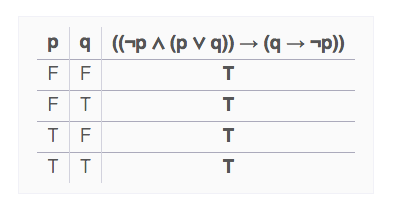
\includegraphics[scale=.5]{../assets/img/3-a.png}
                \end{center}
                \begin{equation*} \begin{split}
                    \tcboxmath{\therefore \, \,  \vDash \varphi}
                \end{split} \end{equation*}

            \item $(p \lor q) \land (p \rightarrow r) \land (q \rightarrow r) \rightarrow r$
                \begin{equation*} \begin{split}
                    \alpha = (p \lor q) \land (p \rightarrow r) \land (q \rightarrow r) \rightarrow r \\
                \end{split} \end{equation*}
                \begin{center}
                    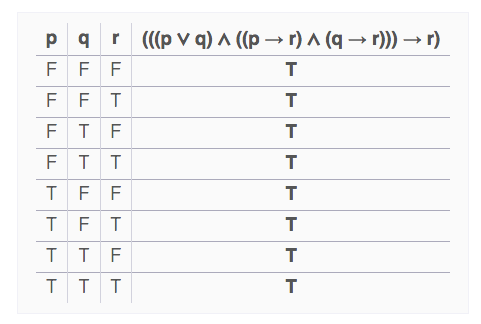
\includegraphics[scale=.5]{../assets/img/3-b.png}
                \end{center}
                \begin{equation*} \begin{split}
                    \tcboxmath{\therefore \, \,  \vDash \alpha}
                \end{split} \end{equation*}
        \end{enumerate}

    \clearpage
    \item Utilizando las leyes de equivalencia de la lógica proposicional,
        muestra que se cumplen las siguientes equivalencias

        \begin{enumerate}
            \item $\neg r \rightarrow b \land \neg b \equiv r$
                \begin{equation*} \begin{split} \begin{aligned}
                    \neg r \rightarrow b \land \neg b &\equiv r \\
                    \neg r \rightarrow (b \land \neg b) &\equiv r \\
                    \neg r \rightarrow 0 &\equiv r \\
                    \neg (\neg r) \lor 0 &\equiv r \\
                    r \lor 0 &\equiv r \\
                    \tcboxmath{r \equiv r} \\
                \end{aligned} \end{split} \end{equation*}

            \item $(p \rightarrow q) \land (p \rightarrow \neg q) \equiv \neg p$
                \begin{equation*} \begin{split} \begin{aligned}
                    (p \rightarrow q) \land (p \rightarrow \neg q) &\equiv \neg p \\
                    (\neg p \lor q) \land (\neg p \lor \neg q) &\equiv \neg p \\
                    \neg p \lor (q \land \neg q) &\equiv \neg p \\
                    \neg p \lor 0 &\equiv \neg p \\
                    \tcboxmath{\neg p \equiv \neg p} \\
                \end{aligned} \end{split} \end{equation*}

            \item $\neg (p \leftrightarrow q) \equiv \neg p \leftrightarrow q$
                \begin{equation*} \begin{split} \begin{aligned}
                    % 1
                    \neg (p \leftrightarrow q)
                        &\equiv
                    \neg p \leftrightarrow q \\
                    % 2
                    \neg ((p \land q) \lor (\neg p \land \neg q))
                        &\equiv
                    (\neg p \land q) \lor (p \land \neg q) \\
                    % 3
                    \neg(p \land q) \land \neg(\neg p \land \neg q)
                        &\equiv
                    (\neg p \land q) \lor (p \land \neg q) \\
                    % 4
                    (\neg p \lor \neg q) \land (p \lor q)
                        &\equiv
                    (\neg p \land q) \lor (p \land \neg q) \\
                    % 5
                    (\neg p \land p) \lor (p \land \neg q) \lor (\neg p \land q) \lor (\neg q \land q)
                        &\equiv
                    (\neg p \land q) \lor (p \land \neg q) \\
                    % 6
                    0 \lor (p \land \neg q) \lor (\neg p \land q) \lor 0
                        &\equiv
                    (\neg p \land q) \lor (p \land \neg q) \\
                    % 7
                    (\neg p \land q) \lor (p \land \neg q)
                        &\equiv
                    (\neg p \land q) \lor (p \land \neg q) \\
                    \tcboxmath{\neg p \leftrightarrow q \equiv \neg p \leftrightarrow q} \\
                \end{aligned} \end{split} \end{equation*}

            \item $p \leftrightarrow q \equiv (p \land q) \lor (\neg p \land \neg q)$
                \begin{equation*} \begin{split} \begin{aligned}
                    % 1
                    p \leftrightarrow q
                        &\equiv
                    (p \land q) \lor (\neg p \land \neg q) \\
                    % 2
                    (p \rightarrow q) \land (q \rightarrow p)
                        &\equiv
                    (p \land q) \lor (\neg p \land \neg q) \\
                    % 3
                    (\neg p \lor q) \land (\neg q \lor p)
                        &\equiv
                    (p \land q) \lor (\neg p \land \neg q) \\
                    % 4
                    (\neg p \land \neg q) \lor (\neg p \land p) \lor (q \land \neg q) \lor (q \land p)
                        &\equiv
                    (p \land q) \lor (\neg p \land \neg q) \\
                    % 5
                    (\neg p \land \neg q) \lor 0 \lor 0 \lor (q \land p)
                        &\equiv
                    (p \land q) \lor (\neg p \land \neg q) \\
                    \tcboxmath{
                        (p \land q) \lor (\neg p \land \neg q)
                            \equiv (p \land q)
                        \lor (\neg p \land \neg q)
                    }
                \end{aligned} \end{split} \end{equation*}
        \end{enumerate}

    \clearpage
    \item Decidir para cada caso si $\mathcal{I} \vDash \phi$
        \begin{enumerate}
            \item $\phi = (p \rightarrow q) \land \neg q \rightarrow r$ con
                $\mathcal{I}(p) = 1$, $\mathcal{I}(q) = 1$ y $\mathcal{I}(r) = 0$
                \begin{equation*} \begin{split} \begin{aligned}
                    \phi &= (p \rightarrow q) \land \neg q \rightarrow r \\
                    \phi &= ((p \rightarrow q) \land \neg q) \rightarrow r \\
                    \phi &= ((1 \rightarrow 1) \land \neg 1) \rightarrow 0 \\
                    \phi &= (1 \land 0) \rightarrow 0 \\
                    \phi &= 0 \rightarrow 0 \\
                    \phi &= 1 \\
                    &\tcboxmath{\therefore \mathcal{I} \vDash \phi}
                \end{aligned} \end{split} \end{equation*}

            \item $\phi = r \rightarrow (p \rightarrow q) \land \neg q$ con
                $\mathcal{I}(p) = 1$, $\mathcal{I}(q) = 0$ y $\mathcal{I}(r) = 0$
                \begin{equation*} \begin{split} \begin{aligned}
                    \phi &= r \rightarrow (p \rightarrow q) \land \neg q \\
                    \phi &= r \rightarrow ((p \rightarrow q) \land \neg q) \\
                    \phi &= 0 \rightarrow ((1 \rightarrow 0) \land \neg 0) \\
                    \phi &= 0 \rightarrow (0 \land 1) \\
                    \phi &= 0 \rightarrow 0 \\
                    \phi &= 1 \\
                    &\tcboxmath{\therefore \mathcal{I} \vDash \phi}
                \end{aligned} \end{split} \end{equation*}

            \item $\phi = (r \rightarrow \neg r) \lor ((p \rightarrow q) \land \neg q)$ con
                $\mathcal{I}(p) = 0$, $\mathcal{I}(q) = 1$ y $\mathcal{I}(r) = 0$
                \begin{equation*} \begin{split} \begin{aligned}
                    \phi &= (r \rightarrow \neg r) \lor ((p \rightarrow q) \land \neg q) \\
                    \phi &= (0 \rightarrow \neg 0) \lor ((0 \rightarrow 1) \land \neg 1) \\
                    \phi &= (0 \rightarrow 1) \lor (1 \land 0) \\
                    \phi &= 1 \lor 0 \\
                    \phi &= 1 \\
                    &\tcboxmath{\therefore \mathcal{I} \vDash \phi}
                \end{aligned} \end{split} \end{equation*}
        \end{enumerate}

    \clearpage
    \item Utilizando interpretaciones, comprobar si se cumplen las afirmaciones:

        \begin{enumerate}
            \item $\{p \land q\} \vDash p \rightarrow q$
                \begin{equation*} \begin{split} \begin{aligned}
                    \text{Sabemos que } \Gamma \vDash A \rightarrow B
                        \text{ si y solo si } \Gamma \cup \{\neg A\} \text{ es insatisfacible.} \\
                    \text{por lo que podemos definir lo anterior como: } \{p \land q, p\} \vDash q\\
                \end{aligned} \end{split} \end{equation*}
                \begin{equation*} \begin{split} \begin{aligned}
                    &\text{\footnotesize{1)} } \mathcal{I}(p \land q) = 1 \\
                    &\text{\footnotesize{2)} } \mathcal{I}(p) = 1 \\
                    &\text{\footnotesize{2)} } \mathcal{I}(q) = 1 \text{ (por \textbf{1} y \textbf{2})}\\
                    &\tcboxmath{\therefore \{p \land q\} \vDash p \rightarrow q}
                \end{aligned} \end{split} \end{equation*}
        \end{enumerate}
\end{enumerate}


\end{document}
